\documentclass[letterpaper, 12pt]{article}

\usepackage[utf8]{inputenc}
\usepackage[english, spanish]{babel}
\usepackage{fullpage}
\usepackage{graphicx}
\usepackage{amsmath}
\usepackage{enumitem}
\usepackage{chngcntr}
\usepackage{setspace}
\usepackage{url}
\usepackage{csquotes}
\usepackage{float}
\usepackage{verbatim}
\usepackage{tabularx}
\usepackage{amsmath}
\usepackage{caption}
\usepackage{bm}
\usepackage{colortbl}
\usepackage{xcolor}

\usepackage{multirow}

% \usepackage{hyperref}

\counterwithin{figure}{section}
\renewcommand{\thesection}{\arabic{section}}
\renewcommand{\thesubsection}{\thesection.\arabic{subsection}}
\renewcommand{\baselinestretch}{1.5}

\usepackage[style=numeric, maxnames=6, minnames=3, backend=biber, parentracker=true, sorting=none]{biblatex}
\DefineBibliographyStrings{english}{%chktex-file 1 chktex-file 6
      andothers = {\em et\addabbrvspace al\adddot}
}
\addbibresource{./Bibliography/bibliography.bib}

\usepackage{array}

\setlength{\parskip}{0pt}

\raggedbottom{}

\newcommand{\bolditalic}[1]{\textbf{\textit{#1}}}

\newcommand{\Celsius}[0]{°$\mathcal{C}$}
\newcommand{\Kelvin}[0]{$\mathcal{K}$}
\newcommand{\Fahrenheit}[0]{°$\mathcal{F}$}

\begin{document}

\begin{titlepage}
      \centering
      
\includegraphics[width=0.3\textwidth]{Images/logo_utb.png}\par\vspace{1cm}
      {\scshape\LARGE Universidad Tecnológica de Bolívar \par}
      \vspace{1cm}

      {\scshape\Large FÍSICA CALOR Y ONDAS \par}
      \vspace{.2cm}

      % chktex-file 8
      {\scshape\Large Grupo 1 \par}
      \vspace{1cm}
      % chktex-file 8
      \slshape {\Large \bfseries{}Informe de Laboratorio No. V\\}
      \slshape {\small \bfseries{}CALOR ESPECÍFICO DE LOS SÓLIDOS}
      \vspace{2cm}

      \slshape {\itshape{} Mauro González, T00067622 \\}
      \slshape {\itshape{} German De Armas Castaño, T00068765 \\}
      \slshape {\itshape{} Angel Vega Rodriguez, T00068186 \\}
      \slshape {\itshape{} Juan Jose Osorio Ariza, T00067316 \\}
      \slshape {\itshape{} Jorge Alberto Rueda Salgado, T00068722 \\}
      \vfill
      Revisado Por \\
      Duban Andres Paternina Verona\\
      {\large \today\par}
\end{titlepage}

% chktex-file 44
% chktex-file 24

% ! ----------------------------------------------------------------------|>
\section{Introducción}

La determinación del calor específico de los sólidos es una
parte fundamental de la termodinámica y juega un papel
esencial en la comprensión de cómo los materiales almacenan
y liberan energía térmica. En esta experiencia de
laboratorio, se lleva a cabo un estudio detallado de la
transferencia de calor entre sólidos y líquidos para
determinar el calor específico de varios materiales. Esto
se logra mediante la medición de cambios de temperatura y
la aplicación de principios termodinámicos fundamentales.
La experimentación práctica en esta área es crucial para la
aplicación de conceptos teóricos en situaciones del mundo
real y es esencial para una amplia gama de campos, desde la
física hasta la ingeniería.

% ! ----------------------------------------------------------------------|>
\section{Objetivos}

% + ----------------------------------------|>
\subsection{Objetivo general}

El objetivo principal de esta práctica de laboratorio es
determinar el calor específico de sólidos utilizando un
enfoque experimental basado en la transferencia de calor y
principios termodinámicos.

% + ----------------------------------------|>
\subsection{Objetivos específicos}

\begin{itemize}[label=$\triangleright$]
      \item Medir la temperatura inicial y final de una mezcla de agua
            y sólidos después de una transferencia de calor controlada.

      \item Determinar la masa equivalente del calorímetro utilizado en
            el experimento.

      \item Calcular el calor específico de los sólidos utilizando los
            datos recopilados y las ecuaciones pertinentes.

      \item Comparar los resultados obtenidos utilizando dos métodos
            diferentes para calcular el calor específico.
\end{itemize}

% ! ----------------------------------------------------------------------|>
\section{Marco Teórico}

% + -------------------------------------------------------------|>
\subsection{Ley cero de la termodinámica~\cite{Fernández}}

Se dice que dos cuerpos están en equilibrio térmico cuando,
al ponerse en contacto, sus variables de estado no cambian.
En torno a esta simple idea se establece la ley cero.

La ley cero de la termodinámica establece que, cuando dos
cuerpos están en equilibrio térmico con un tercero, estos
están a su vez en equilibrio térmico entre sí.

% ! ----------------------------------------------------------------------|>
\section{Montaje Experimental}

\begin{figure}[H]
      \begin{center}
            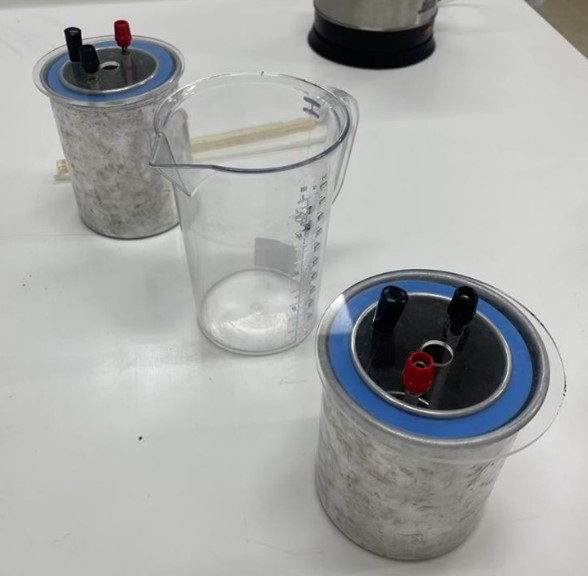
\includegraphics[width=.5\linewidth]{./Images/Montaje1.jpg}
            \caption{}
      \end{center}
\end{figure}

\begin{figure}[H]
      \begin{center}
            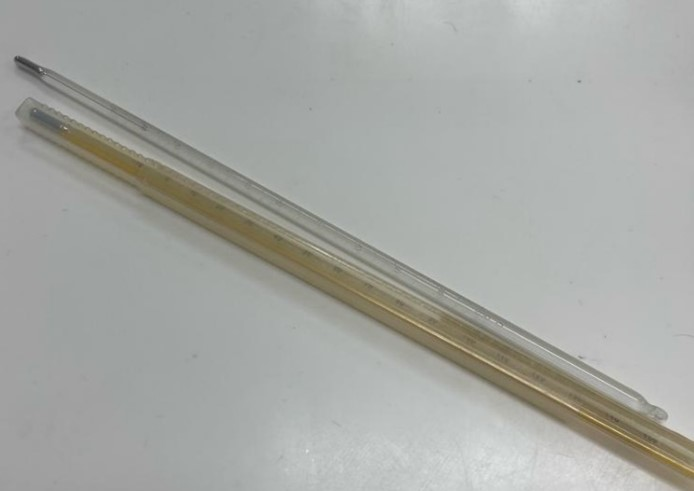
\includegraphics[width=.5\linewidth]{./Images/Montaje2.jpg}
            \caption{}
      \end{center}
\end{figure}

\begin{figure}[H]
      \begin{center}
            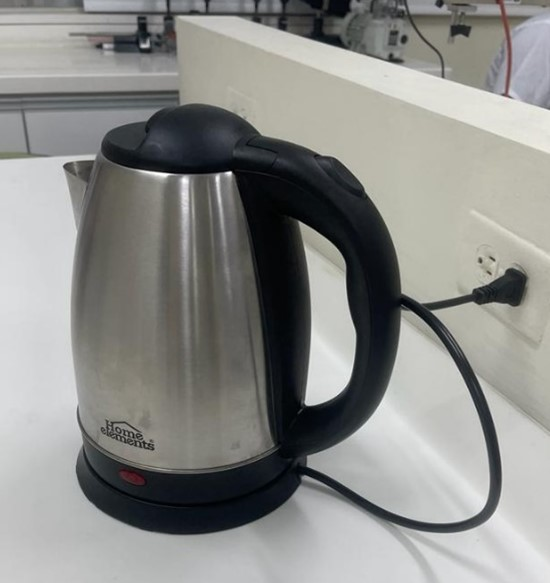
\includegraphics[width=.5\linewidth]{./Images/Montaje3.jpg}
            \caption{}
      \end{center}
\end{figure}

\begin{figure}[H]
      \begin{center}
            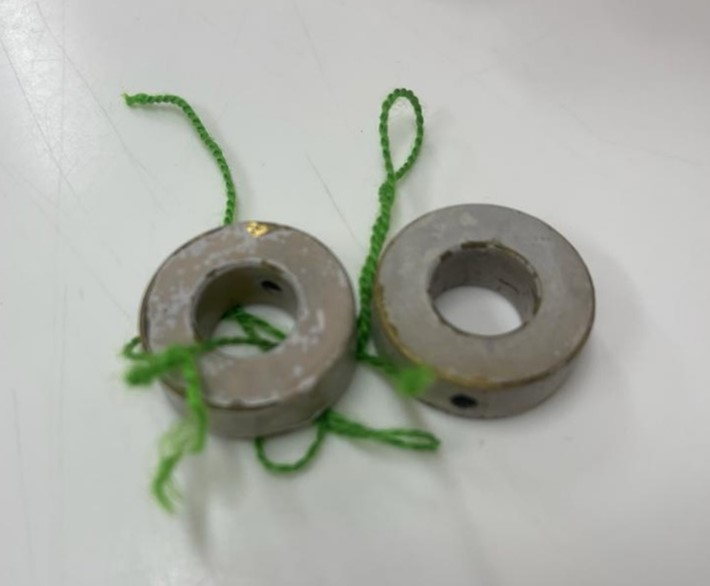
\includegraphics[width=.5\linewidth]{./Images/Montaje4.jpg}
            \caption{}
      \end{center}
\end{figure}

Equipo utilizado:

\begin{itemize}
      \item Vaso de Dewar con tapa (calorímetro).

      \item Bloque o gránulos de cobre, aluminio o Hierro.

      \item Termómetro –10 C a +110 °C o sensor de temperatura NiCr-Ni.

      \item Generador de vapor, 550 W / 220 V.

      \item Aparatos de calefacción.

      \item Vaso de precipitados, 400 -600 ml
\end{itemize}

% ! ----------------------------------------------------------------------|>
\section{Datos Experimentales}

En esta experiencia realizamos un proceso para determinar
el equivalente en agua del calorímetro $m_k$ y el calor
específico de sólidos. Primero, se mezcló agua en el
calorímetro y se midió su temperatura inicial. Luego, se
añadió agua calentada al calorímetro y se registró la
temperatura de equilibrio. Para el calor específico de
sólidos, se midió la masa del sólido, se calentó con agua y
se registraron temperaturas. Luego, se transfirió el sólido
al calorímetro y se monitoreó la temperatura.
Permitiéndonos obtener los siguientes resultados.

\begin{table}[H]
      \begin{center}
            \begin{tabularx}{.9\linewidth}{|>{\centering\arraybackslash}X|>{\centering\arraybackslash}X|>{\centering\arraybackslash}X|>{\centering\arraybackslash}X|}
                  \hline
                  \multirow{3}{*}{Cuerpo} & \multirow{3}{*}{Masa (Kg)} & Temperaturas iniciales $T_0$ Y T~(\Celsius) & Temperatura final $T_e$~(\Celsius) \\\hline

                  M                       & 0,25                       & 28                                          & 40                                 \\\hline

                  m                       & 0,08                       & 92                                          & 40                                 \\\hline
            \end{tabularx}
      \end{center}
\end{table}

\begin{table}[H]
      \begin{center}
            \begin{tabularx}{.9\linewidth}{|>{\centering\arraybackslash}X|>{\centering\arraybackslash}X|>{\centering\arraybackslash}X|>{\centering\arraybackslash}X|}
                  \hline
                  Sustancia   & Masa (Kg) & $T_0$\Celsius & $T_m$ de equilibrio \\\hline

                  Calorímetro & 0,25      & \dots         & 31                  \\\hline

                  Agua        & 0.2       & 28            & 31                  \\\hline

                  Solido      & 0,0964    & 91            & 31                  \\\hline
            \end{tabularx}
      \end{center}
\end{table}

% ! ----------------------------------------------------------------------|>
\section{Análisis de datos}

% + -------------------------------------------------------------|>
\subsection{Análisis}

% * --------------------------------------------------------|>
\subsubsection{}

Ecuación 2:~$Q_1 = C_1 m_1 (T_1 - T_M)$, Ecuación 3:~$Q_2 =
      C_2 m_2 (T_2 - T_M)$, Ecuación 4:~$Q_1 + Q_2$

Reemplazando (2) y (3) en (4), obtenemos,

$C_1 m_1 (T_1 - T_M) + C_2 m_2 (T_2 - T_M) = 0$

Luego se despeja $C_1$

\begin{equation*}
      \begin{gathered}
            C_1 m_1 (T_1 - T_M) = -C_2 m_2 (T_2 - T_M) \\
            C_1 = \frac{- C_2 m_2 (T_2 - T_M)}{m_1 (T_1 - T_M)} \\
            C_1 = C_2 \frac{m_2 (T_M - T_2)}{m_1 (T_1 - T_M)}~\surd
      \end{gathered}
\end{equation*}

% * --------------------------------------------------------|>
\subsubsection{}

Ecuación 7:~$Q_2 = C_2 (m_2 + m_k)(T_M - T_2)$, Ecuación
2:~$Q_1 = C_1 m_1 (T_1 - T_M)$, Ecuación 4:~$Q_1 + Q_2 = 0$

Reemplazando (2) y (7) en (4)

$C_2 (m_2 + m_k)(T_M T_2) + C_1 m_1 (T_1 - T_M) = 0$

Luego se despeja $C_1$ de la ecuación

\begin{equation*}
      \begin{gathered}
            C_1 = \frac{- C_2(m_2 + m_k)(T_M - T_2)}{m_1 (T_1 - T_M)} \\
            C_1 = C_2 \frac{(m_2 + m_k)(T_M - T_2)}{m_1 (T_1 - T_M)}~\surd
      \end{gathered}
\end{equation*}

% * --------------------------------------------------------|>
\subsubsection{}

Ecuación 10:~$m_K = \frac{m (T - T_e)}{T_e - T_o}$

Reemplazando los valores, $m_K = \frac{0.08 (92 - 40)}{40 -
            28} = 0.097 Kg$

% * --------------------------------------------------------|>
\subsubsection{}

Utilizando la ecuación,

\begin{equation}
      C_{1} = C_{2} \frac{m_{2} (T_{m} - T_{2})}{m_1 (T_{1} - T_{m})}
      \label{eq:calor_especifico_1}
\end{equation}

Donde,

\begin{itemize}[label=$\triangleright$]
      \item $m_{1}$: masa del sólido,
      \item $C_{1}$: su calor especifico
      \item $m_{2}$: masa del agua,
      \item $C_{2}$: el calor específico de calor del agua,
      \item $T_{1}$: temperatura de la sustancia,
      \item $T_{2}$: temperatura del agua,
      \item $T_{m}$: temperatura común.
\end{itemize}

El calor específico del agua es de: \hfill{} \break{}
$C_{2} = 4.19\frac{J}{K\cdot KG}$

\smallskip

Conversiones:

\begin{itemize}[label=$\triangleright$]
      \item $m_{1}$: $96.4$~g = $0.0964$~kg
      \item $m_{2}$: $200$~g = $0.20$~kg
      \item $T_{m}$: $31$\Celsius = $304.15$~\Kelvin
      \item $T_{1}$: $91$\Celsius = $364.15$~\Kelvin
      \item $T_{2}$: $28$\Celsius = $301.15$~\Kelvin
\end{itemize}

\begin{equation*}
      \begin{gathered}
            C_{1} = 4.19 \frac{J}{K \cdot Kg} \times \frac{0.20 Kg (304.15~\mathcal{K} - 301.15~\mathcal{K})}{0,0964 Kg(364.15~\mathcal{K} - 304.15~\mathcal{K})} \\
            C_{1} = 0.435 \frac{J}{K \cdot Kg}
      \end{gathered}
\end{equation*}

% * --------------------------------------------------------|>
\subsubsection{}

\begin{equation}
      C_{1} = C_{2} \frac{(m_{2} + m_{k})(T_{M} - T_{2})}{m_{1}(T_{1} - T_{M})}
      \label{eq:calor_especifico_2}
\end{equation}

Masa del calorímetro:

\begin{equation}
      m_{k} = \frac{m(T - T_{e})}{T_{e} - T_{0}} - M
      \label{eq:masa_calorimetro}
\end{equation}

Donde,

\begin{itemize}[label=$\triangleright$]
      \item $T_{0}$: temperatura del agua en el calorímetro sin calentar
      \item $T$: temperatura del agua calentada
      \item $T_{e}$: temperatura en equilibrio
      \item $M$: gramos de agua iniciales
      \item $m$: gramos de agua añadidos
\end{itemize}

Conversiones:

\begin{itemize}
      \item $M$: $250$g = $0.25$~Kg
      \item $m$: $80$g = $0.08$~Kg
      \item $T_{0}$: $28$\Celsius = $301.15$~\Kelvin
      \item $T$: $92$\Celsius = $365.15$~\Kelvin
      \item $T_{e}$: $40$\Celsius = $313.15$~\Kelvin
\end{itemize}

\begin{equation*}
      \begin{gathered}
            m_k = \frac{0,08 Kg(365.15~\mathcal{K} - 313.15~\mathcal{K})}{313.15~\mathcal{K} - 301.15~\mathcal{K}} \\
            m_k = 0.097 Kg
      \end{gathered}
\end{equation*}

\begin{equation*}
      \begin{gathered}
            C_{1} = 4.19 \frac{J}{K \cdot Kg} \times \frac{(0.020 Kg + 0.097 Kg)(304.15~\mathcal{K} - 301.15~\mathcal{K})}{0,0964 Kg(364.15~\mathcal{K} - 304.15~\mathcal{K})} \\
            C_{1} = 0.645 \frac{J}{K \cdot Kg}
      \end{gathered}
\end{equation*}

% * --------------------------------------------------------|>
\subsubsection{}

\begin{itemize}[label=$\triangleright$]
      \item En el punto 4, se calculó el calor específico ($C_1$)
            utilizando la ecuación (\ref{eq:calor_especifico_1}).\@{}El
            valor obtenido fue aproximadamente $0.435 \frac{J}{K \cdot
                        Kg}$.

      \item En el punto 5, se volvió a calcular el calor específico
            ($C_1$) utilizando la ecuación
            (\ref{eq:calor_especifico_2}), teniendo en cuenta la masa
            del calorímetro. El valor obtenido fue aproximadamente
            $0.435 \frac{J}{K \cdot Kg}$.

            En el punto 5, se considera la masa del calorímetro, que es
            de $0.25$ kg. El calorímetro es la parte del sistema que
            almacena el calor y, por lo tanto, afecta la cantidad de
            calor que puede absorber o liberar durante un cambio de
            temperatura. Cuando se calcula el calor específico (C1)
            utilizando la ecuación HERE, la masa total del sistema
            ($m_2$ + $m_k$) en el denominador es la suma de la masa del
            calorímetro ($m_k$) y la masa de agua añadida ($m_2$). Esto
            significa que el calorímetro en sí mismo contribuye a la
            capacidad térmica total del sistema. Por lo tanto, el
            resultado de C1 se ve influenciado por la masa del
            calorímetro y cómo esta afecta la absorción de calor
            durante el experimento.

            En resumen, los dos métodos utilizados para determinar el
            calor específico
            (\ref{eq:calor_especifico_1})~(\ref{eq:calor_especifico_2})
            proporcionaron resultados ligeramente diferentes. Esto
            puede deberse a las diferencias en las ecuaciones y a la
            consideración de la masa del calorímetro en el punto 5.
            Considerar la masa del calorímetro es crucial, ya que
            afecta directamente el resultado final del cálculo del
            calor específico ($C_1$). La masa del calorímetro se suma a
            la masa total del sistema y contribuye a su capacidad
            térmica, lo que hace que el resultado de $C_1$ sea más
            preciso y realista en condiciones experimentales.
\end{itemize}

% ! ----------------------------------------------------------------------|>
\section{Conclusiones}

En esta experiencia de laboratorio, se llevaron a cabo
mediciones precisas de la transferencia de calor entre
sólidos y agua. Se determinaron los calores específicos de
los sólidos utilizando dos métodos diferentes, uno que
considera el calor absorbido por el agua y otro que tiene
en cuenta la masa equivalente del calorímetro. Se
encontraron diferencias en los resultados obtenidos por
estos métodos, lo que demuestra la importancia de
considerar la contribución del calorímetro en el proceso.

Estos experimentos proporcionaron una comprensión práctica
de los conceptos fundamentales de la termodinámica y
demostraron la relación entre la masa, la temperatura y el
calor específico de los sólidos. Además, destacaron la
necesidad de la precisión en la medición y la importancia
de la calibración adecuada de los instrumentos utilizados
en experimentos de transferencia de calor.

\printbibliography

\end{document}